\documentclass[slidestop]{beamer}
\usepackage{beamerthemesplit}
\usepackage{graphics}
\usepackage{pstricks}

\graphicspath{{./}}

\title{The Libre-SOC Hybrid 3D CPU}
\author{Luke Kenneth Casson Leighton}


\begin{document}

\frame{
   \begin{center}
    \huge{The Libre-SOC Hybrid 3D CPU}\\
    \vspace{32pt}
    \Large{Augmenting the OpenPOWER ISA}\\
    \Large{to provide 3D and Video instructions}\\
    \Large{(properly and officially) and make a GPU}\\
    \vspace{24pt}
    \Large{XDC2020}\\
    \vspace{16pt}
    \large{Sponsored by NLnet's PET Programme}\\
    \vspace{6pt}
    \large{\today}
  \end{center}
}


\frame{\frametitle{Why another SoC?}

 \begin{itemize}
   \item Intel Management Engine, Apple QA issues, Spectre\vspace{6pt}
   \item Endless proprietary drivers, "simplest" solution: \\
         License proprietary hard macros (with proprietary firmware)\\
   		 Adversely affects product development cost\\
   		due to opaque driver bugs (Samsung S3C6410 / S5P100)
   		 \vspace{6pt}
   \item Alternative: Intel and Valve-Steam collaboration\\
         "Most productive business meeting ever!"\\
         https://tinyurl.com/valve-steam-intel
		\vspace{6pt}
   \item Because for 30 years I Always Wanted To Design A CPU
		\vspace{6pt}
   \item Ultimately it is a strategic \textit{business} objective to
         develop entirely Libre hardware, firmware and drivers.
  \end{itemize}
}


\frame{\frametitle{Why OpenPOWER?}

\vspace{15pt}

 \begin{itemize}
   \item Good ecosystem essential\\
   		 linux kernel, u-boot, compilers, OSes,\\
   		 Reference Implementation(s)\vspace{10pt}
   \item Supportive Foundation and Members\\
   		 need to be able to submit ISA augmentations\\
   		 (for proper peer review)\vspace{10pt}
   \item No NDAs, full transparency must be acceptable\\
	     due to being funded under NLnet's PET Programme\vspace{10pt}
   \item OpenPOWER: established for decades, excellent Foundation,\\
   	     Microwatt as Reference, approachable and friendly.
  \end{itemize}
}


\frame{\frametitle{What goes into a typical SoC?}
\vspace{9pt}
 \begin{itemize}
   \item 15 to 20mm BGA package: 2.5 to 5 watt power consumption\\
   		heat sink normally not required (simplifies overall design)
   		\vspace{10pt}
   \item Fully-integrated peripherals (not Northbridge/Southbridge)\\
         USB, HDMI, RGB/TTL, SD/MMC, I2C, UART, SPI, GPIO etc. etc. 
         \vspace{10pt}
   \item Built-in GPU (shared memory bus, 3rd party licensed) \vspace{10pt}
   \item Build-in VPU (likewise)\vspace{10pt}
   \item Target price between \$2.50 and \$30 depending on market\\
         Radically different from IBM POWER9 Core (200 Watt)
         \vspace{10pt}
  \end{itemize}
}



\frame{\frametitle{Simple SBC-style SoC}

\begin{center}
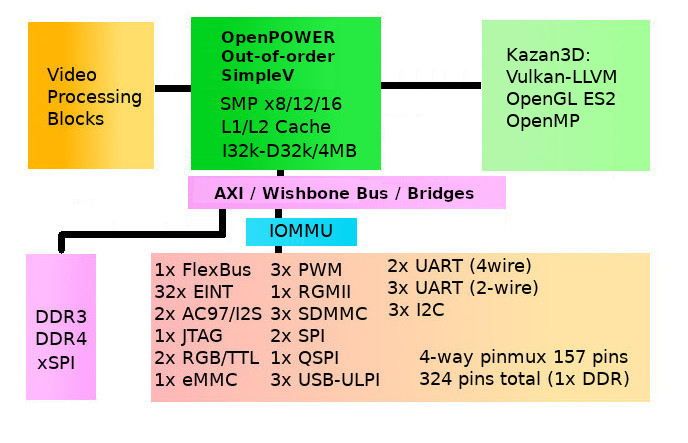
\includegraphics[width=0.9\textwidth]{shakti_libre_soc.jpg}
\end{center}

}

\frame{\frametitle{What's different about Libre-SOC?}

 \begin{itemize}
   \item Hybrid - integrated.  The CPU \textit{is} the GPU.\\
         The GPU \textit{is} the CPU.  The VPU \textit{is} the CPU.\\
         \textit{There is No Separate VPU/GPU Pipeline}\\
   		  \vspace{9pt}
   \item written in nmigen (a python-based HDL).  Not VHDL\\
   		  not Verilog (definitely not Chisel3/Scala)\\
   		  This is an extremely important strategic decision.\\
   		  \vspace{9pt}
   \item Simple-V Vector Extension.  See `SIMD Considered harmful'.\\
   		  https://tinyurl.com/simd-considered-harmful\\   
   		SV effectively a "hardware for-loop" on standard scalar ISA\\
   		(conceptually similar to Zero-Overhead Loops in DSPs)
   		  \vspace{9pt}
  \end{itemize}
}

\frame{\frametitle{Hybrid Architecture: Augmented 6600}

 \begin{itemize}
   \item CDC 6600 is a design from 1965.  The \textit{augmentations} are not.\\
   		 Help from Mitch Alsup includes \textit{precise exceptions}, \\
   		 multi-issue and more. Academic literature on 6600 utterly misleading.
   		6600 Scoreboards completely underestimated (Seymour Cray and
   		James Thornton
   		solved problems they didn't realise existed elsewhere!)
   \item Front-end Vector ISA, back-end "Predicated (masked) SIMD"\\
         nmigen (python OO) strategically critical to achieving this.
   \item Out-of-order combined with Simple-V allows scalar operations\\
         at the developer end to be turned into SIMD at the back-end\\
         \textit{without the developer needing to do SIMD}
   \item IEEE754 sin / cos / atan2, Texturisation opcodes, YUV2RGB\\
   		 all automatically vectorised.
  \end{itemize}
}

\frame{\frametitle{Why nmigen?}

 \begin{itemize}
   \item Uses python to build an AST (Abstract Syntax Tree).
         Actually hands that over to yosys (to create ILANG file)
         after which verilog can (if necessary) be created
   \item Deterministic synthesiseable behaviour (Signals are declared
         with their reset pattern: no more forgetting "if rst" block).
   \item python OO programming techniques can be deployed.  classes
         and functions created which pass in parameters which change
         what HDL is created (IEEE754 FP16 / 32 / 64 for example)
   \item python-based for-loops can e.g. read CSV files then generate
         a hierarchical nested suite of HDL Switch / Case statements
         (this is how the Libre-soc PowerISA decoder is implemented)
   \item extreme OO abstraction can even be used to create "dynamic
         partitioned Signals" that have the same operator-overloaded
         "add", "subtract", "greater-than" operators
   
  \end{itemize}
}

\frame{\frametitle{Why another Vector ISA? (or: not-exactly another)}

 \begin{itemize}
   \item Simple-V is a 'register tag' system.  \textit{There are no opcodes}\\
   		 SV 'tags' scalar operations (scalar regfiles) as 'vectorised'
   \item (PowerISA SIMD is around 700 opcodes, making it unlikely to be
    	 able to fit a PowerISA decoder in only one clock cycle)
   \item Effectively a 'hardware sub-counter for-loop': pauses the PC\\
         then rolls incrementally through the operand register numbers\\
         issuing \textit{multiple} scalar instructions into the pipelines\\
         (hence the reason for a multi-issue OoO microarchitecture)
   \item Current \textit{and future} PowerISA scalar opcodes inherently
   	 	 \textit{and automatically} become 'vectorised' by SV without
   	 	 needing an explicit new Vector opcode.
   \item Predication and element width polymorphism are also 'tags'.
         elwidth polymorphism allows for FP16 / 80 / 128 to be added to
         the ISA \textit{without modifying the ISA}
   
  \end{itemize}
}

\frame{\frametitle{Quick refresher on SIMD}

 \begin{itemize}
   \item SIMD very easy to implement (and very seductive)
   \item Parallelism is in the ALU
   \item Zero-to-Negligeable impact for rest of core
  \end{itemize}
  Where SIMD Goes Wrong:\vspace{6pt}
   \begin{itemize}
   \item See "SIMD instructions considered harmful"
   https://sigarch.org/simd-instructions-considered-harmful
   \item Setup and corner-cases alone are extremely complex.\\
         Hardware is easy, but software is hell.\\
         strncpy VSX patch for POWER9: 250 hand-written asm lines!\\
         (RVV / SimpleV strncpy is 14 instructions)
   \item O($N^{6}$) ISA opcode proliferation (1000s of instructions)\\
         opcode, elwidth, veclen, src1-src2-dest hi/lo
  \end{itemize}
}

\begin{frame}[fragile]
\frametitle{Simple-V ADD in a nutshell}

\begin{semiverbatim}
function op\_add(rd, rs1, rs2, predr) # add not VADD!
  int i, id=0, irs1=0, irs2=0;
  for (i = 0; i < VL; i++)
    if (ireg[predr] & 1<<i) # predication uses intregs
       ireg[rd+id] <= ireg[rs1+irs1] + ireg[rs2+irs2];
    if (reg\_is\_vectorised[rd] )  \{ id += 1; \}
    if (reg\_is\_vectorised[rs1])  \{ irs1 += 1; \}
    if (reg\_is\_vectorised[rs2])  \{ irs2 += 1; \}
\end{semiverbatim}

  \begin{itemize}
   \item Above is oversimplified: Reg. indirection left out (for clarity).
   \item SIMD slightly more complex (case above is elwidth = default)
   \item Scalar-scalar and scalar-vector and vector-vector now all in one
   \item OoO may choose to push ADDs into instr. queue (v. busy!)
  \end{itemize}
\end{frame}

\begin{frame}[fragile]
\frametitle{Predication-Branch (overload meaning of "branch")}

\begin{semiverbatim}
s1 = reg\_is\_vectorised(src1);
s2 = reg\_is\_vectorised(src2);
if (!s2 && !s1) goto branch;
for (int i = 0; i < VL; ++i)
  if (cmp(s1 ? reg[src1+i]:reg[src1],
          s2 ? reg[src2+i]:reg[src2])
         ireg[rs3] |= 1<<i;
\end{semiverbatim}

  \begin{itemize}
   \item Above is oversimplified (case above is elwidth = default)
   \item If s1 and s2 both scalars, Standard branch occurs
   \item Predication stored in integer regfile as a bitfield
   \item Scalar-vector and vector-vector supported
   \item Overload Branch immediate to be predication target rs3
  \end{itemize}
\end{frame}

\begin{frame}[fragile]
\frametitle{Register element width and packed SIMD}

\begin{semiverbatim}
    typedef union \{
       uint8\_t  actual\_bytes[8]; // actual SRAM bytes
       uint8\_t  b[]; // array of type uint8\_t
       uint16\_t s[]; // etc
       uint32\_t i[];
       uint64\_t l[];
    \} reg\_t;
    
    reg\_t int\_regfile[128];
\end{semiverbatim}

 \begin{itemize}
   \item Regfile is treated (sort-of) as a byte-level SRAM
   \item Each "register" starts at an 8-byte offset into SRAM
   \item requires byte-level "select" lines on SRAM
  \end{itemize}

\end{frame}

\frame{\frametitle{Register element width and packed SIMD}

 \begin{itemize}
   \item default: elements behave as defined by the standard ISA
   \item override for Integer operations: 8/16/32 bit SIMD
   \item override for IEEE754 FP: FP16/FP32 (and later FP80 or FP128)
   \item Effectively "typecasts" regfile to union of arrays
   \item Does not require modification of ISA!  This is "tagging"\\
         (similar to the `Mill' ISA)
   \item FPADD64 RT, RA, RB becomes `actually please do FP16'\\
         (but without needing to add an actual FPADD16 opcode)
   \item Note: no zeroing unless explicitly requested!\\
         (unused elements e.g. VL=3 when elwidth=16 are
         predicated out: int\_regfile[RA].s[3] is not zero'd)
  \end{itemize}

}

\frame{\frametitle{Additional Simple-V features}

 \begin{itemize}
   \item "fail-on-first" (POWER9 VSX strncpy segfaults on boundary!)
   \item "Twin Predication" (covers VSPLAT, VGATHER, VSCATTER, VINDEX etc.)
   \item SVPrefix: 16-bit and 32-bit prefix to scalar operations\\
   	     (SVP-64 allows more extensive "tag" augmentation)
   \item VBLOCK: a VLIW-like context.  Allows space for `swizzle' tags
         and more.  Effectively a "hardware compression algorithm" for ISAs.
   \item Ultimate goal: cut down I-Cache usage, cuts down on power
   \item Typical GPU has its own I-Cache and small shaders.\\
        \textit{We are a Hybrid CPU/GPU: I-Cache is not separate!}
   \item Needs to go through OpenPOWER Foundation `approval'         
  \end{itemize}
}


\frame{\frametitle{Summary}

 \begin{itemize}
   \item Goal is to create a mass-volume low-power embedded SoC suitable
         for use in netbooks, chromebooks, tablets, smartphones, IoT SBCs.
   \item No way we could implement a project of this magnitude without
         nmigen (being able to use python OO to       HDL)
   \item Collaboration with OpenPOWER Foundation and Members absolutely
         essential. No short-cuts.  Standards to be developed and ratified
         so that everyone benefits.
   \item Working on the back of huge stability of POWER ecosystem
   \item Greatly simplified open 3D and Video drivers reduces product
         development costs for customers
   \item It also happens to be fascinating, deeply rewarding technically
         challenging, and funded by NLnet
         
  \end{itemize}
}


\frame{
  \begin{center}
    {\Huge The end\vspace{15pt}\\
		   Thank you\vspace{15pt}\\
		   Questions?\vspace{15pt}
	}
  \end{center}
  
  \begin{itemize}
	\item Discussion: http://lists.libre-soc.org
	\item Freenode IRC \#libre-soc
	\item http://libre-soc.org/
	\item http://nlnet.nl/PET
  \end{itemize}
}


\end{document}
